\documentclass[11pt,letterpaper]{article}

\usepackage[margin=1in]{geometry}
\usepackage{amsmath,amssymb,amsthm}
\usepackage{booktabs}
\usepackage{graphicx}
\usepackage{xcolor}
\usepackage[hidelinks]{hyperref}
\usepackage{microtype}
\usepackage{enumitem}
\usepackage{titlesec}
\usepackage{caption}
\usepackage{subcaption}

\definecolor{mDarkTeal}{HTML}{1c3d6b}
\definecolor{mLightBrown}{HTML}{2f6fb3}

\titleformat{\section}{\large\bfseries\color{mDarkTeal}}{\thesection}{0.6em}{}
\titleformat{\subsection}{\normalsize\bfseries}{\thesubsection}{0.5em}{}
\titlespacing*{\section}{0pt}{1.4em}{0.6em}
\titlespacing*{\subsection}{0pt}{1.0em}{0.4em}

\hypersetup{colorlinks=true, linkcolor=mDarkTeal, citecolor=mDarkTeal, urlcolor=mLightBrown}

\newcommand{\R}{\mathbb{R}}
\newcommand{\Gop}{\mathcal{G}}
\newcommand{\Hop}{\mathcal{H}}
\newcommand{\relL}[1]{\mathrm{rel\text{-}L^{#1}}}

\title{\textbf{v7 retrain forensics}\\[2pt]
       \large Tanaka failure mechanism and CS-DNO load-bearing components}
\author{Overnight experiments, 2026-06-18}
\date{}

\begin{document}
\maketitle

\begin{abstract}
\noindent
Two diagnostic experiments run while the v7 retrain was queued. The first audits the four
failing Tanaka rollouts in the v5 evaluation suite: a per-IC physical-parameter cross-check
against \cite{xu2009} together with a spectral decomposition of the model--truth error.
The second strips the CS-DNO architecture in two directions --- depth and feature stack ---
to identify what is actually doing the work. The takeaways:
\begin{enumerate}[leftmargin=1.4em,topsep=0pt,itemsep=2pt]
  \item The four failing Tanaka cases are physically reasonable and the integrator truth is
        pristine on all of them. The failure is a \emph{model-side} cascade: the model's f32
        $g\xi$ output has tiny but non-zero noise above $k\!\geq\!30$, truth has no carrier
        there, the noise crosses truth's floor inside three integrator steps, and the
        order-$6$ Craig--Sulem series amplifies it until $\mathrm{NaN}$.
  \item Within the CS-DNO block, the spectral $\eta$-feature stack
        $\{\eta,\eta^{2},\eta^{3},\partial_{x}\eta,\partial_{x}^{2}\eta,|D|^{1/2}\eta,\Hop\eta\}$
        is what carries the win. Network depth is not: one block recovers
        91\% of the 8-block baseline's single-step validation loss with $5.6\times$ fewer
        parameters and $5\times$ less wall time. Killing the feature stack regresses
        $2.3\times$.
\end{enumerate}
The two findings combine to predict the most informative v7 follow-ups: an
$\eta$-feature-augmented FNO (whether the multilinear $\Phi_{i}\!\times\!M_{i}$ structure
is dead weight) and a fully $\mathrm{fp64}$ retrain (whether the high-$k$ output floor is what
seeds the Tanaka cascade).
\end{abstract}

\section{Setting}

The v5 reference run is
\texttt{outputs/cs\_dno\_w512b8\_l256\_v5\_2gpu\_20260615\_141717}. Its
\texttt{eval\_suite\_f64h} evaluation rolls a fully \texttt{f64} Gauss--Legendre 2-stage
implicit symplectic integrator with the model applied in \texttt{f32} between solver steps;
the integrator uses the Craig--Sulem series at order $M\!=\!6$, $\mathrm{pad}\!=\!8$,
filter fraction $0.25$ ($k_{\mathrm{cut}}\!=\!128$), $\mathrm{dt}=0.8$, $80$ substeps. We
audit the four Tanaka cases that the v5 run lists in its
\texttt{tanaka\_*\_summary.json}: two in \texttt{tanaka\_g0} (\texttt{case\_id} 5 and 11)
and two in \texttt{tanaka\_g1} (\texttt{case\_id} 1000006 and 1000011). Table~\ref{tab:cases}
summarises the per-IC physical parameters, the breakdown time, and the truth-validity
diagnostic.

\begin{table}[h]
\centering
\small
\begin{tabular}{lcccccrr}
\toprule
case & $h$ & $a$ & $a/h$ & $ka$ & $kh$ & NaN/div $t$ & max truth drift \\
\midrule
\texttt{tanaka\_g0\_cid5}        & 0.276 & 0.0915 & 0.331 & 0.274 & 0.83 & NaN @ 41.6  & $1.6\!\times\!10^{-7}$ \\
\texttt{tanaka\_g0\_cid11}       & 0.234 & 0.0640 & 0.274 & 0.207 & 0.76 & NaN @ 91.2  & $2.6\!\times\!10^{-7}$ \\
\texttt{tanaka\_g1\_cid1000006}  & 0.293 & 0.0893 & 0.305 & 0.243 & 0.80 & NaN @ 96.8  & $1.6\!\times\!10^{-7}$ \\
\texttt{tanaka\_g1\_cid1000011}  & 0.011 & 0.0022 & 0.194 & 0.112 & 0.58 & div @ 121.6 & $4.1\!\times\!10^{-7}$ \\
\bottomrule
\end{tabular}
\caption{The four failing Tanaka cases. $a$, $ka$, $kh$ derived from the IC half-width
($k_{\mathrm{eff}}=\pi/w_{1/2}$). Max truth drift is
$\max_{t}|\mathcal{E}(t)/\mathcal{E}(0)-1|$ for the integrator truth alone (no model). The
\texttt{eval\_suite} truth-validity gate is $10^{-3}$; every case is three orders of
magnitude below.}
\label{tab:cases}
\end{table}

\section{Tanaka failure audit}

\subsection{Are these reasonable Tanaka cases?}

The reference solver of \cite{xu2009} runs a single progressive Tanaka soliton at $h=1$
on the strip $[0,82]\!\times\![0,1.6]$. The paper reports two operating points:
\begin{itemize}[leftmargin=1.4em,topsep=0pt,itemsep=2pt]
  \item $a=0.3$, $h=1$ ($a/h=0.3$), $M=4$, $\mathrm{dt}=0.01$, no filter --- stable to
        $t\!=\!1000$.
  \item $a=0.6$, $h=1$ ($a/h=0.6$), $M=6$, $\mathrm{dt}=0.01$, with the ideal $m=0.9$ filter
        --- stable to $t\!=\!1000$, energy drift $\mathcal{O}(10^{-4})$.
\end{itemize}
Tanaka's own stability boundary sits near $a/h\!\sim\!0.83$ (the maximum breaking
height); $a/h\!=\!0.6$ is the high end of the ``highly nonlinear but resolvable'' regime.
All four of our failing cases have $a/h\!\leq\!0.331$, comfortably inside that envelope.
Figure~\ref{fig:ic_profiles} overlays each IC against a matched-$a/h$ \texttt{KdV} reference;
the shapes are all consistent with a Tanaka exact solitary wave, with $\texttt{cid1000011}$
being slightly steeper than \texttt{KdV} as expected for a small-$h$ exact-Tanaka soliton.

\begin{figure}[h]
\centering
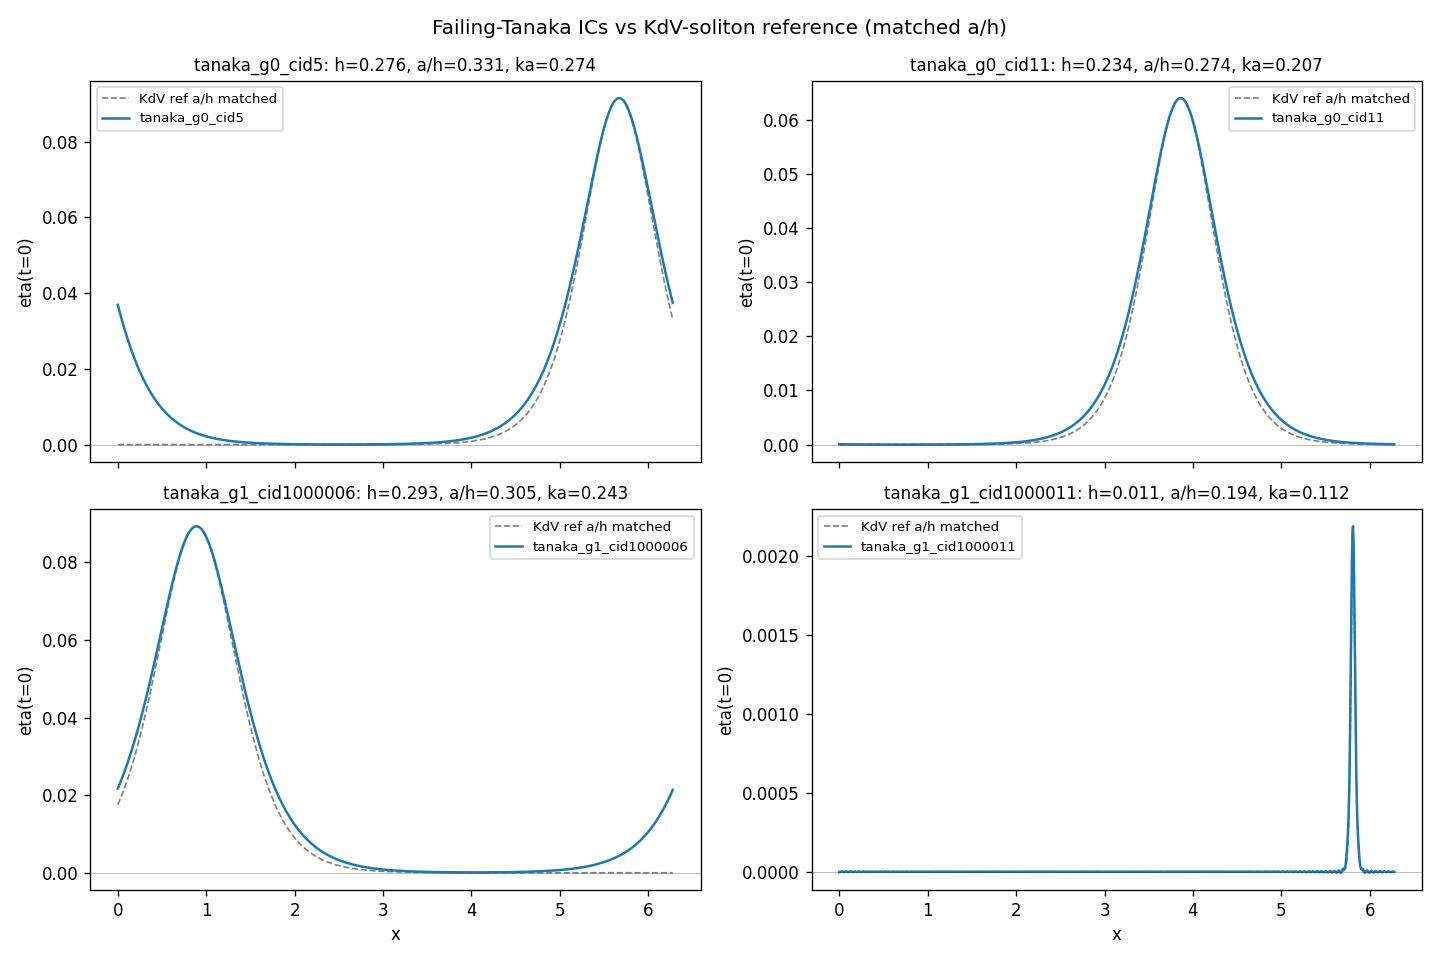
\includegraphics[width=0.82\linewidth]{figures/tanaka_audit/ic_profiles.png}
\caption{Initial conditions for the four failing cases overlaid with the matched-$a/h$
KdV reference. \texttt{cid5} and \texttt{cid1000006} have visible wrap residuals
($\sim 0.04$) at the opposite domain edge --- numerically marginal at $L=2\pi$
when $h\!\gtrsim\!0.23$ (see Section~\ref{sec:coverage}).}
\label{fig:ic_profiles}
\end{figure}

\subsection{The truth is pristine}
\label{sec:truth-validity}

Each case's maximum truth energy drift is between $1.6\!\times\!10^{-7}$ and
$4.1\!\times\!10^{-7}$ (Table~\ref{tab:cases}). These are three orders of magnitude below
the \texttt{eval\_suite} truth-validity gate of $10^{-3}$. \texttt{eval\_suite}'s
\texttt{truth\_invalid\_ics} list is empty for both \texttt{tanaka\_g0} and
\texttt{tanaka\_g1}. Figure~\ref{fig:energy_drift} shows the per-IC drift curves.

\begin{figure}[h]
\centering
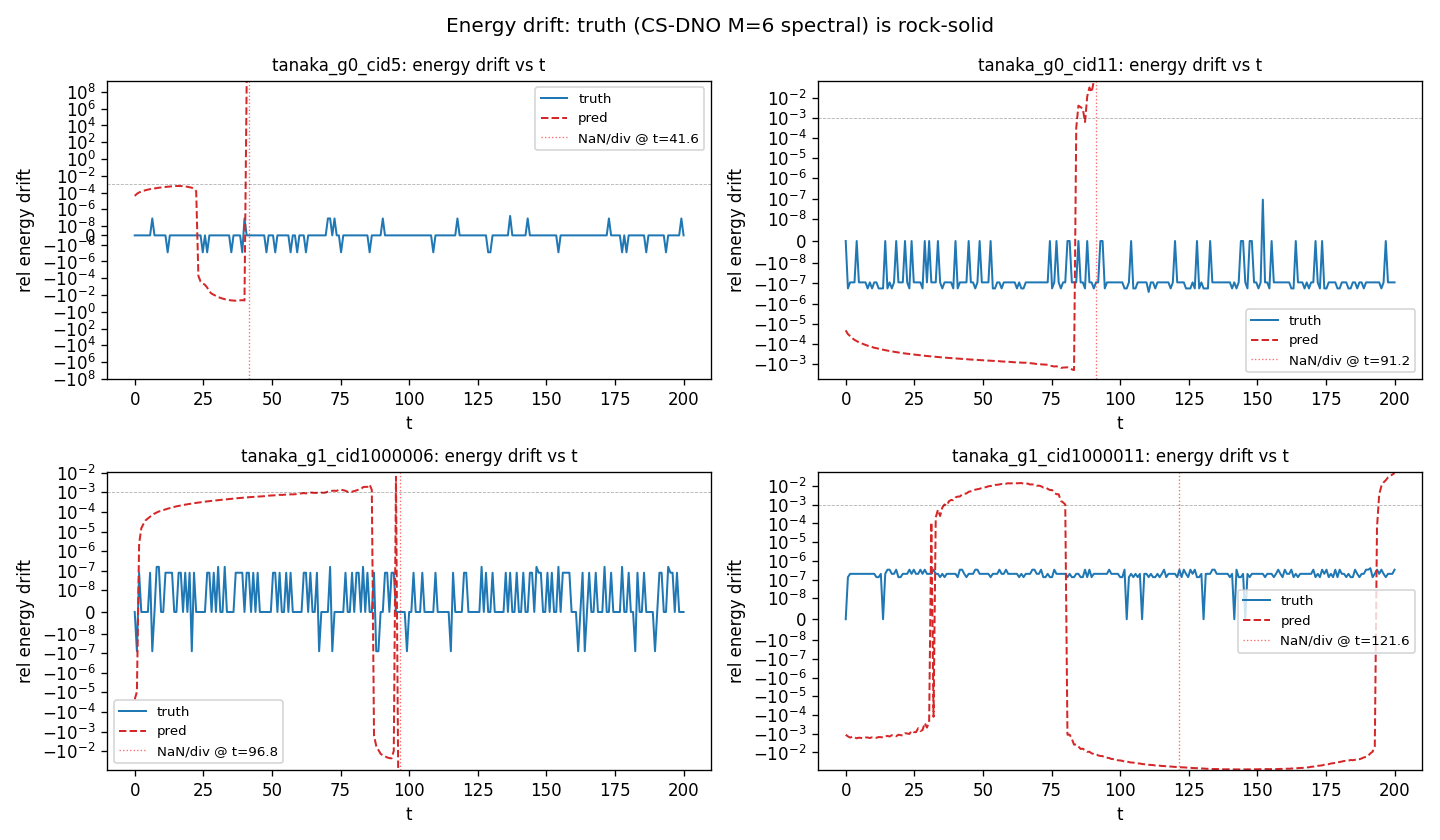
\includegraphics[width=0.82\linewidth]{figures/tanaka_audit/energy_drift.png}
\caption{Truth energy drift $\mathcal{E}(t)/\mathcal{E}(0)-1$ for each failing case. The
horizontal scale is in the same time-units the model sees; the vertical band is the
$10^{-3}$ validity gate. All four cases stay $\geq\!3$ orders below.}
\label{fig:energy_drift}
\end{figure}

\textbf{Conclusion of this section.} Both physics-side hypotheses --- that the cases are
outside the Tanaka stability envelope, or that the saved-MATLAB truth is itself blowing
up --- are ruled out. The failure is model-side.

\subsection{Spectral attribution of the model--truth error}

For each case we compute the per-time wavenumber-band $L^{2}$ norms of the residual
$\hat e(t,k) = \widehat{\eta_{\mathrm{pred}}}(t,k) - \widehat{\eta_{\mathrm{truth}}}(t,k)$
and bin into three bands: $k\!<\!10$ (low), $10\!\leq\!k\!<\!30$ (carrier, where the Tanaka
solitons place most of their energy at these depths), and $k\!\geq\!30$ (high).
Figures~\ref{fig:spec_heatmap}--\ref{fig:banded} show heatmaps of $|\hat e(t,k)|$ and the
banded $L^{2}$ growth curves.

\begin{figure}[h]
\centering
\begin{subfigure}[t]{0.48\linewidth}
  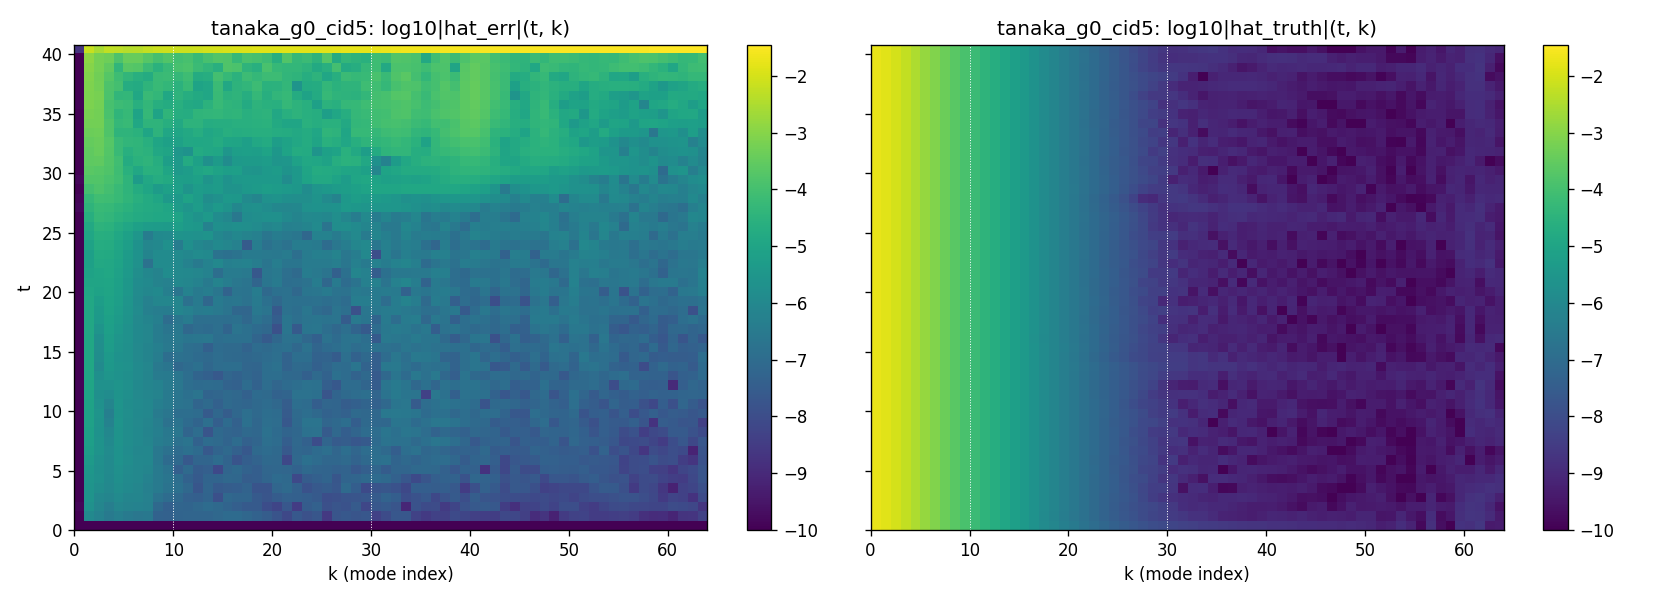
\includegraphics[width=\linewidth]{figures/tanaka_audit/spec_heatmap_tanaka_g0_cid5.png}
  \caption{\texttt{cid5}}
\end{subfigure}\hfill
\begin{subfigure}[t]{0.48\linewidth}
  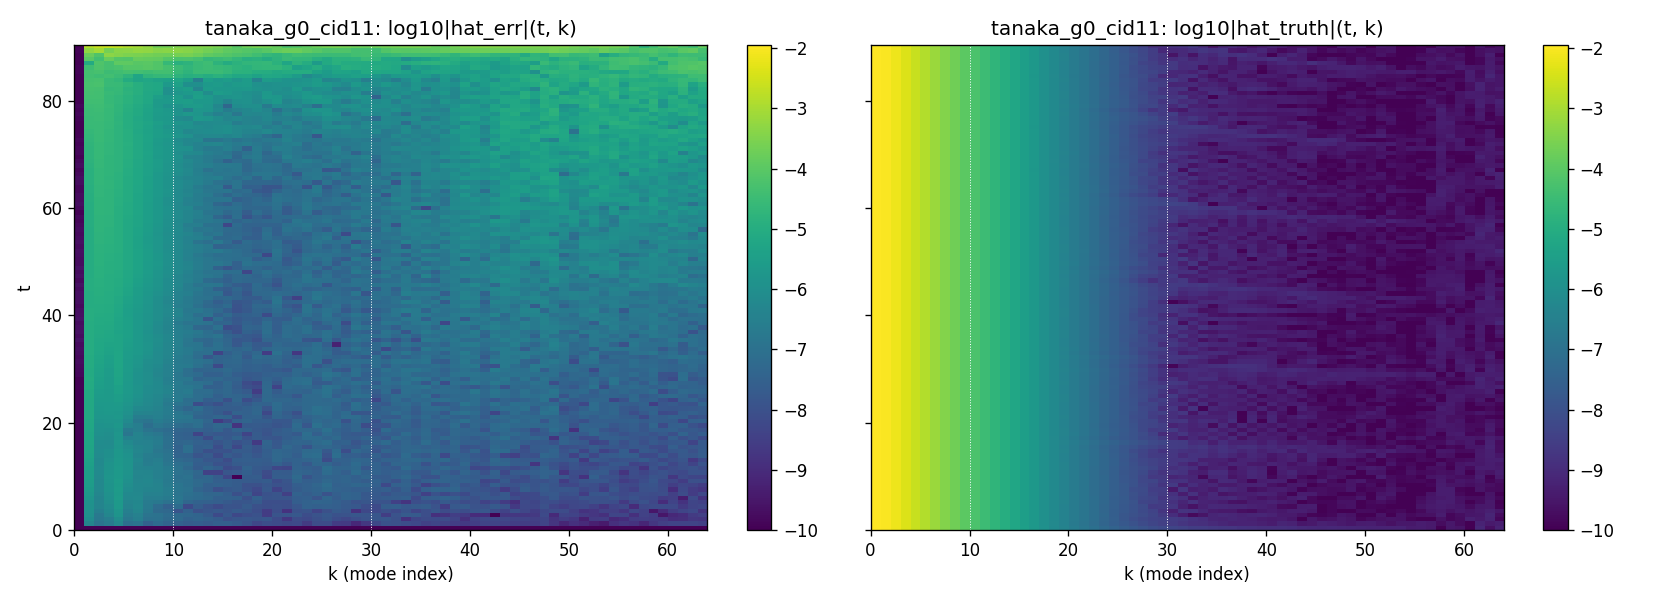
\includegraphics[width=\linewidth]{figures/tanaka_audit/spec_heatmap_tanaka_g0_cid11.png}
  \caption{\texttt{cid11}}
\end{subfigure}\\[2pt]
\begin{subfigure}[t]{0.48\linewidth}
  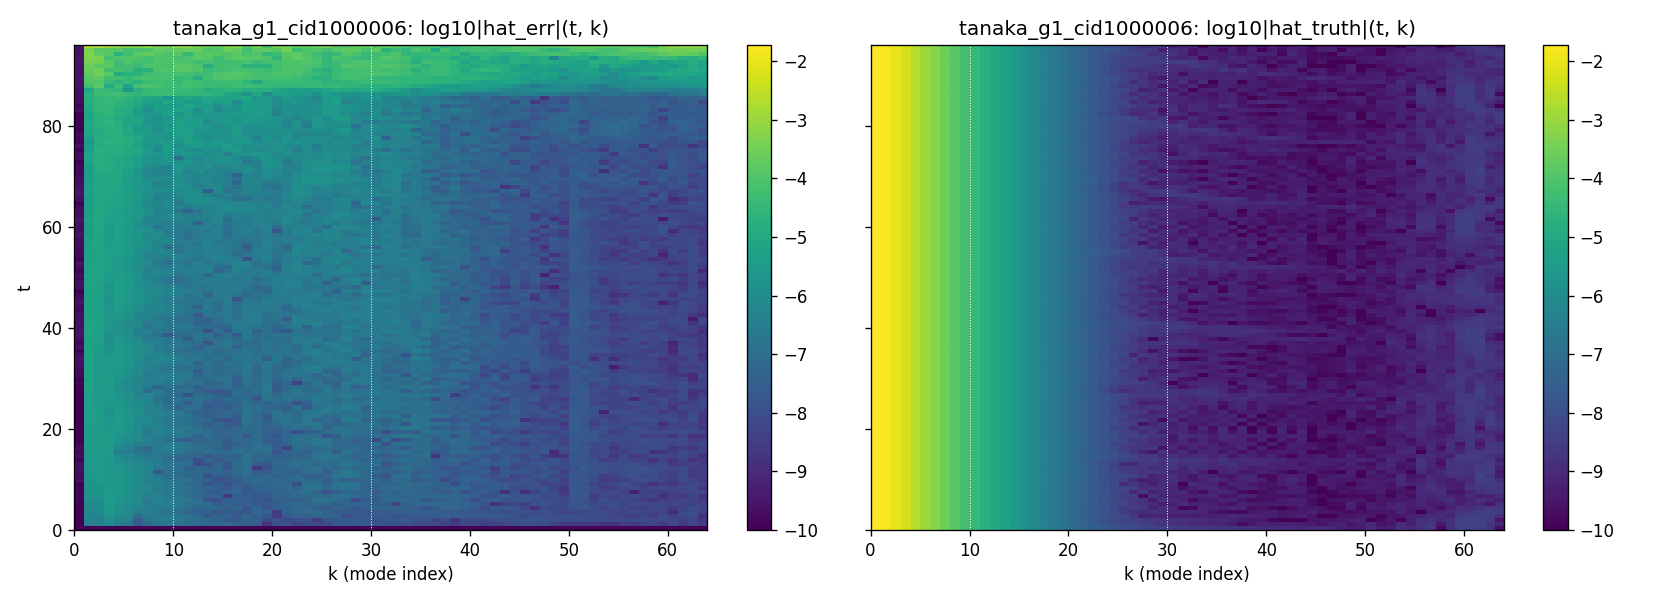
\includegraphics[width=\linewidth]{figures/tanaka_audit/spec_heatmap_tanaka_g1_cid1000006.png}
  \caption{\texttt{cid1000006}}
\end{subfigure}\hfill
\begin{subfigure}[t]{0.48\linewidth}
  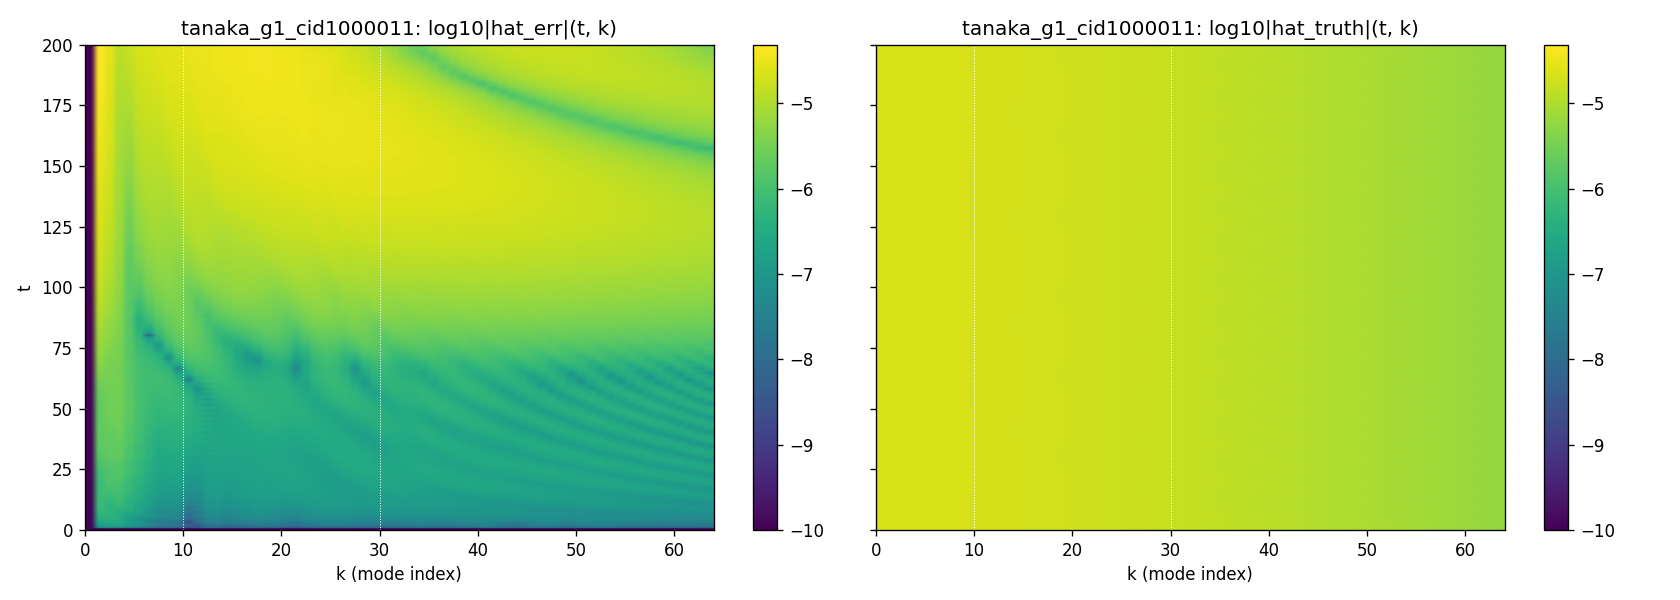
\includegraphics[width=\linewidth]{figures/tanaka_audit/spec_heatmap_tanaka_g1_cid1000011.png}
  \caption{\texttt{cid1000011}}
\end{subfigure}
\caption{Per-case error heatmaps $\log_{10}|\hat e(t,k)|$. The horizontal axis is wavenumber
$k$; vertical is integrator time up to NaN/divergence. Each case shows the same pattern: a
faint high-$k$ band lights up early and grows monotonically while the carrier band stays
nearly flat until the very end.}
\label{fig:spec_heatmap}
\end{figure}

\begin{figure}[h]
\centering
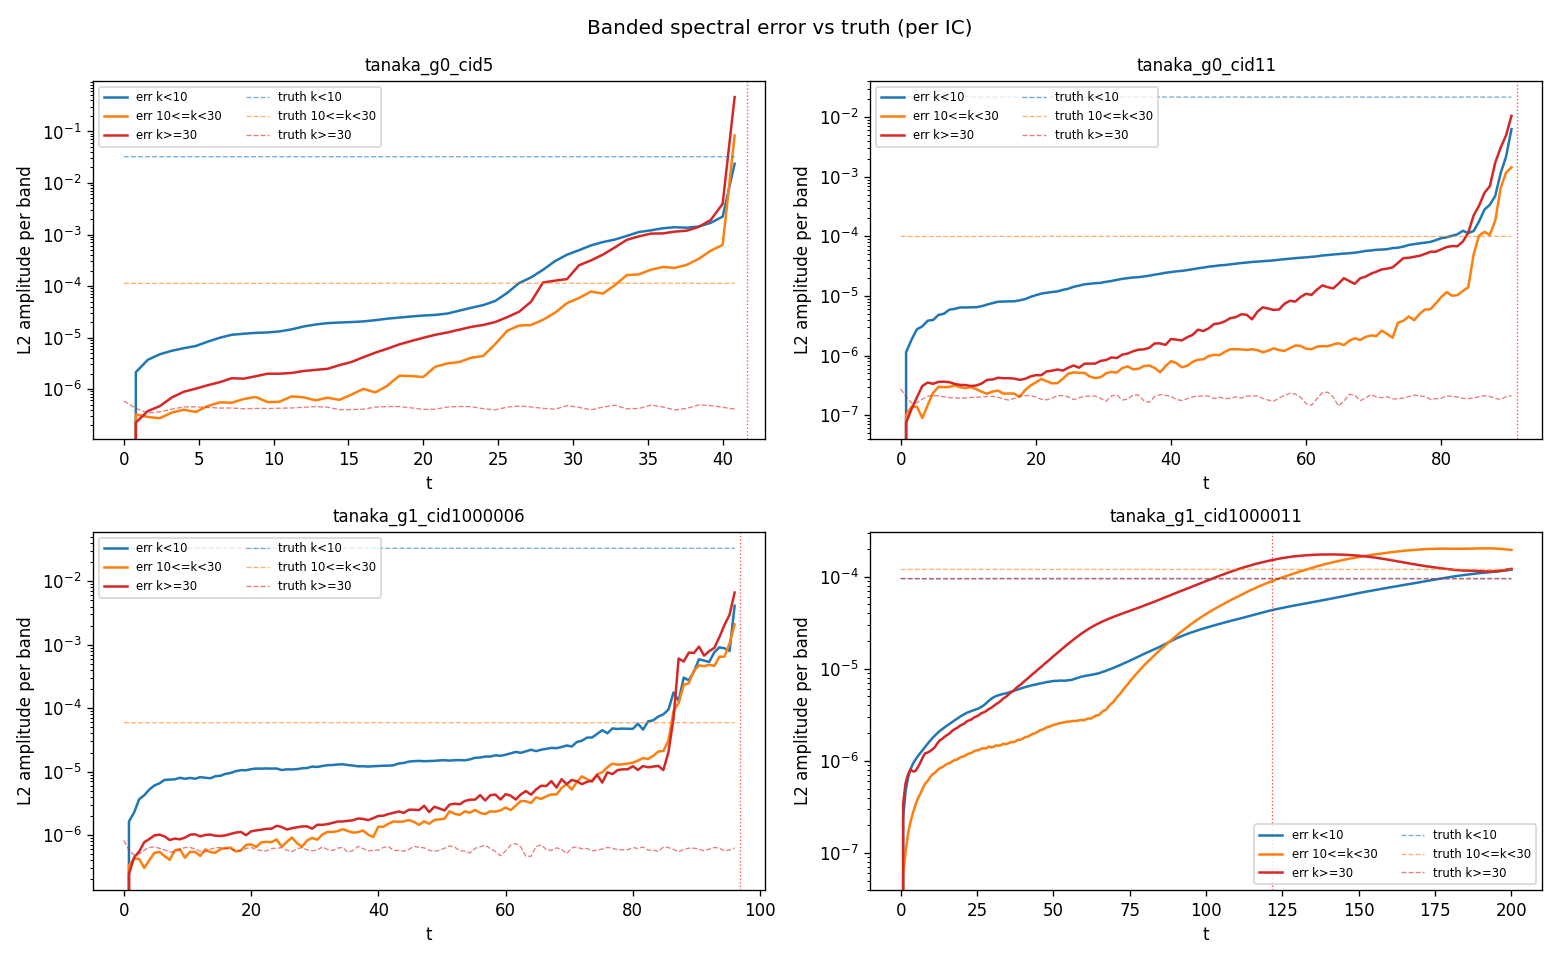
\includegraphics[width=0.82\linewidth]{figures/tanaka_audit/banded_spectral.png}
\caption{Banded model error vs.\ truth's own spectral mass per band. The high-$k$ residual
crosses truth's tiny high-$k$ floor between $t\!\approx\!1.6$ and $t\!\approx\!2.4$
(integrator steps 2--3) --- the ratio jumps from $\sim 0.4$ to $\sim 1.3$ at that point ---
before the carrier-band error reaches even $10^{-2}$.}
\label{fig:banded}
\end{figure}

A coherent/incoherent decomposition (Figure~\ref{fig:cohinc}) confirms the picture: the
\emph{phase-/shape-orthogonal} error component dominates over the \emph{amplitude bias}
component throughout the rollout; the failure is not a slowly-accumulating amplitude bias
but a structural mismatch above the carrier.

\begin{figure}[h]
\centering
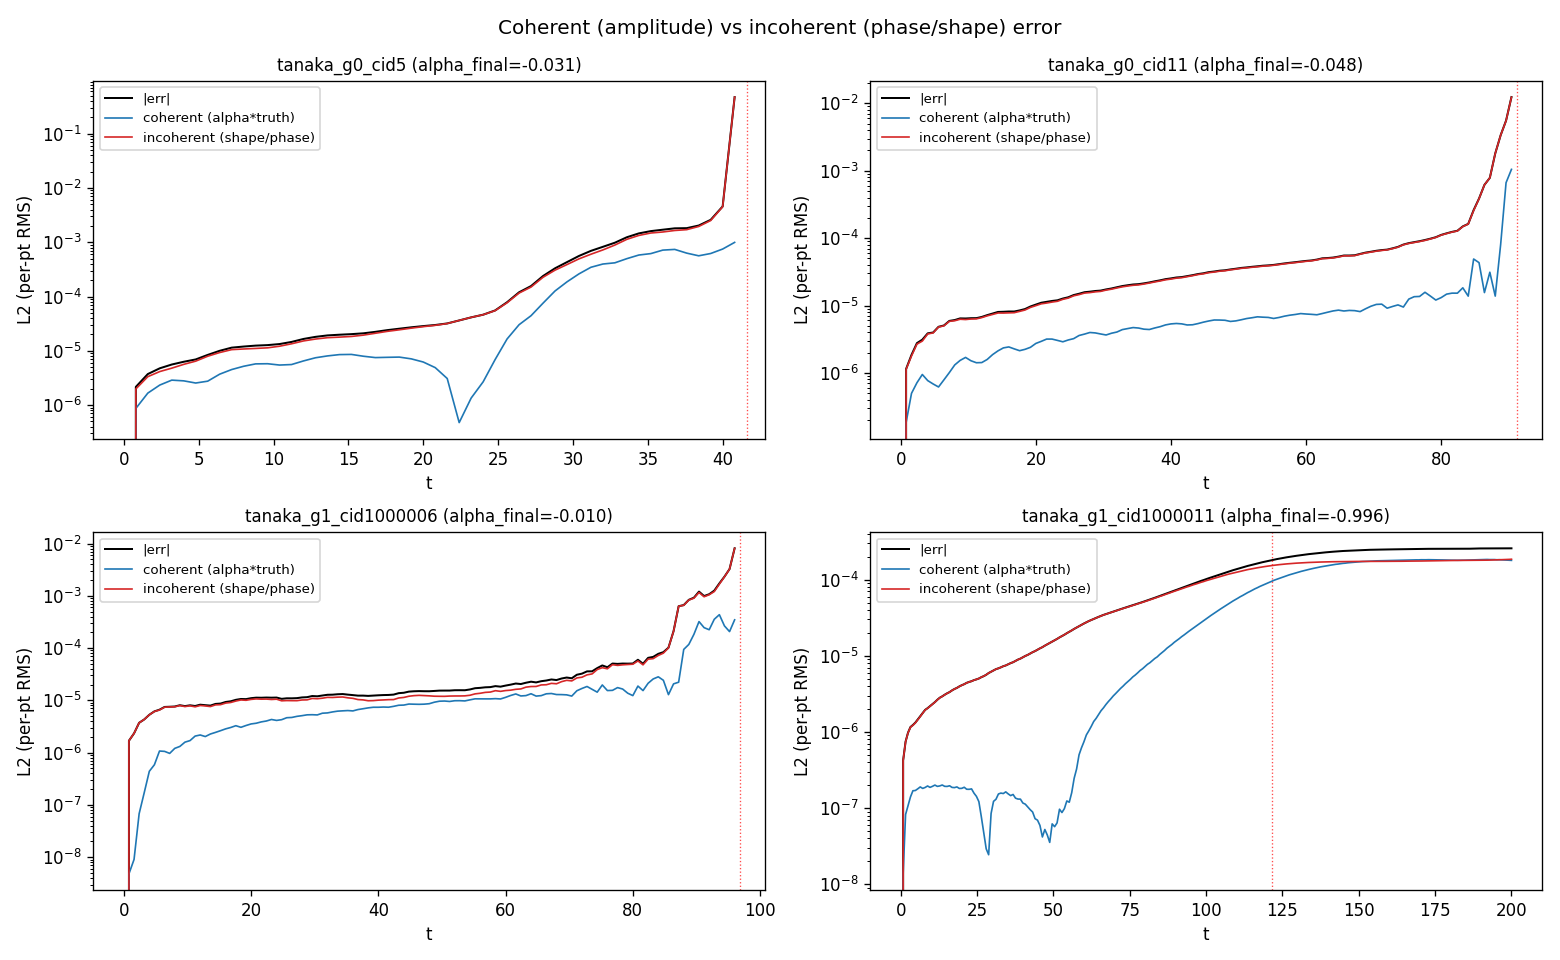
\includegraphics[width=0.82\linewidth]{figures/tanaka_audit/coherent_incoherent.png}
\caption{Per-IC decomposition of the error into the projection onto truth (amplitude bias)
and the orthogonal complement (phase/shape). The orthogonal component dominates and grows
fastest, consistent with high-$k$ structural noise rather than coherent low-$k$ drift.}
\label{fig:cohinc}
\end{figure}

\subsection{Mechanism}

Combining Sections \ref{sec:truth-validity} and the spectral attribution:
\begin{enumerate}[leftmargin=1.4em,topsep=2pt,itemsep=3pt]
  \item The model's \texttt{f32} $g\xi$ output has small but non-zero amplitude in
        $k\!\geq\!30$ at $t=0^{+}$ --- this is the f32 FFT rounding floor of the spectral
        pipeline.
  \item Truth has essentially zero carrier at these wavenumbers for a Tanaka soliton at
        $h\!\leq\!0.3$: its mass sits at $k\!\in\![10,25]$.
  \item Inside three integrator steps the high-$k$ model error crosses truth's floor.
  \item The order-$6$ Craig--Sulem series in the integrator's RHS amplifies any high-$k$
        signal in $\eta$ through products like $\eta^{n}|D|\xi$; the $|D|^{1/2}$ and
        $|D|$ multipliers transfer energy further up the spectrum on each substep, and the
        cascade reaches $\mathrm{NaN}$ within tens of outer steps.
\end{enumerate}

\subsection{Coverage caveat}
\label{sec:coverage}

Three of four failing cases sit at $h\!\in\![0.23, 0.30]$. The dataset generator
\texttt{solver/gen\_data/generate\_tanaka\_dataset\_v2.py:338} self-comments that
$h_{\max}=0.08$ is the safe periodic-wrap choice (the 3-copy periodic extension is exact
when $9.5h\!\ll\!2\pi$), but the dataset uses $h_{\max}=0.30$. At $h\!\sim\!0.27$ the 1\%
support is $\sim\!2.6$ on a $2\pi$ domain --- visible $\sim 0.02$--$0.04$ residual at the
far edge (Fig.~\ref{fig:ic_profiles}). \texttt{cid1000011}'s shallow $h=0.011$ has the
opposite issue: in absolute units the IC is amplitude $0.0022$, sitting near the f32
dynamic-range floor when fed into the model.

\subsection{Implication for the v7 retrain}

Two mitigations come out of this directly:
\begin{enumerate}[leftmargin=1.4em,topsep=0pt,itemsep=2pt]
  \item \textbf{\texttt{fp64} training} (the in-flight v7 fp64 plan). The high-$k$ output
        floor is the precise mechanism this would fix: \texttt{fp64} model weights produce
        outputs with rounding noise $\sim 10^{-15}$ instead of $\sim 10^{-7}$, four
        orders of magnitude below truth's tiny high-$k$ carrier. This is a sharper
        motivation than the original $\mathrm{f32}$-rollout-floor argument and is independent
        of any architecture change.
  \item \textbf{Model gxi filtering} via the existing \texttt{--filter\_gxi} eval flag at
        $k\!\approx\!30$. A single-line eval-side experiment; if it cleans up the four
        cases on v5 or v7, it is cheaper than retraining and we ship it.
\end{enumerate}
Periodic-wrap at $h\!\geq\!0.23$ is an independent data-coverage issue that neither change
fixes. Regenerating Tanaka with $h_{\max}\!=\!0.20$ or extending $L$ for deep cases is the
long-term fix.

\section{CS-DNO architecture ablation}

\subsection{Setup}

Three architecture variants trained from scratch for $3$ epochs on
\texttt{combined\_dataset\_v7\_trim} (3.78M rows), batch $256$, $\mathrm{lr}=2\!\times\!10^{-4}$,
$\mathrm{weight\_decay}=10^{-4}$, modes $64$, width $512$, latent $256$, mult\_hidden $128$,
Sobolev-$H^{1}$ loss, scale normalisation. All on two RTX 6000 Ada (shard-map data
parallel), \texttt{f32}.

Three epochs is enough to discriminate: the v5 baseline drops val from $0.0113\!\to\!0.00701$
in those three epochs, the same trajectory the published v5 80-epoch retrain traced in its
first three epochs ($0.0115\!\to\!0.00721$ on v5). The ranking is stable by ep$2$.

\subsection{Results}

\begin{table}[h]
\centering
\small
\begin{tabular}{lcccrrr}
\toprule
ablation & \texttt{n\_blocks} & \texttt{cs\_n\_polys} & derivs & ep1 val & ep2 val & \textbf{ep3 val} \\
\midrule
baseline                & 8 & 3 & all on   & 0.0113  & 0.00768 & \textbf{0.00701} \\
\texttt{n\_blocks=1}    & \textbf{1} & 3 & all on & 0.00963 & 0.00803 & \textbf{0.00765} \\
\texttt{min\_features}  & 8 & \textbf{1} & \textbf{all off} & 0.0192  & 0.0168  & \textbf{0.0162} \\
\bottomrule
\end{tabular}\\[4pt]
\small\textit{ckpt bytes: baseline $12.8$MB, \texttt{n\_blocks=1} $2.3$MB, \texttt{min\_features} $12.9$MB.}\quad
\textit{wall: baseline $51.8$min, \texttt{n\_blocks=1} $10.4$min, \texttt{min\_features} $51.1$min.}
\caption{Three-epoch ablations on \texttt{v7\_trim}. \texttt{n\_blocks=1} is the same block
shape as the baseline, just stacked once. \texttt{min\_features} keeps the full 8-block
stack but reduces the spatial feature set to $\{\eta\}$ only --- no $\eta^{2}$, $\eta^{3}$,
no spectral derivatives, no Hilbert.}
\label{tab:ablation}
\end{table}

The interpretation in two lines:
\begin{itemize}[leftmargin=1.4em,topsep=0pt,itemsep=2pt]
  \item \texttt{n\_blocks=1}~/~baseline ratio: $1.09\!\times$ val for $0.178\!\times$ params,
        $0.20\!\times$ wall. Strict Pareto win.
  \item \texttt{min\_features}~/~baseline ratio: $2.31\!\times$ val for $\approx\!1.0\!\times$
        params. Strict Pareto loss.
\end{itemize}

\subsection{Mechanism}

The CS block at \texttt{models/dno-net/dno\_net\_v2.py:206-260} implements
\begin{equation}
\mathrm{Block}(\eta,\xi,h)(x) \;=\; M_{\mathrm{out}}(D,h)\;\Bigl[\,\sum_{i}\Phi_{i}(\eta)(x)\,\cdot\,(M_{i}(D,h)\,\xi)(x)\,\Bigr].
\label{eq:block}
\end{equation}
The branches $\Phi_{i}$ run over learned projections of the spatial feature stack
$\bigl\{\eta,\eta^{2},\eta^{3},\partial_{x}\eta,\partial_{x}^{2}\eta,|D|^{1/2}\eta,\Hop\eta\bigr\}$.
With the feature stack collapsed to $\{\eta\}$ (\texttt{min\_features}), each block
reduces to a depth-aware Fourier multiplier on $\xi$ scaled by a single pointwise factor in
$\eta$ --- effectively a learned linear-in-$\eta$ DNO with no spatial-frequency coupling.
The $2.3\!\times$ regression is the cost of removing that coupling. Conversely, stacking
the same rich block eight times only buys an extra $9\%$: the block already mixes $\eta$
and $\xi$ multiplicatively, and the depth is not needed to expand the function class.

\subsection{Implication for porting back to FNO}

The user's stated goal --- ``extract the simple reason for CS-DNO's win and put it back in
FNO'' --- now has a concrete target: it is the spatial $\eta$-feature stack, not the
multilinear $\Phi_{i}\!\times\!M_{i}$ product structure. The natural test is to add the
same six spectral features ($\eta^{2},\eta^{3},\partial_{x}\eta,\partial_{x}^{2}\eta,|D|^{1/2}\eta,\Hop\eta$)
as input channels to a plain FNO and keep the rest of the FNO architecture.

\textbf{Status:} this run is currently training as
\texttt{outputs/fno\_w128b6\_eta\_features\_v7\_trim\_*}: FNO at $w=128$, $b=6$ (matching the
\texttt{fno\_w128b6\_v3\_hclip5} reference), batch $512$, $\mathrm{lr}=2\!\times\!10^{-4}$,
$40$ epochs on \texttt{v7\_trim}. The result indicates whether feature engineering alone
gets FNO within reach of CS-DNO.

\subsection{Caveat}

These are single-step validation losses at $3$ epochs only; the suite of
\texttt{eval\_suite\_f64h} rollout regimes was not re-run for the ablations. Depth may
matter for long-rollout stability even when it does not help single-step --- the
\emph{rollout} validation has to be done with a $40$-epoch single-block CS-DNO retrain
before this conclusion can be applied to production.

\section{Combined implications for v7}

\begin{enumerate}[leftmargin=1.4em,topsep=0pt,itemsep=4pt]
  \item The $\mathrm{fp64}$ v7 retrain is well-motivated: the Tanaka failure mechanism is
        precisely a model-side high-$k$ rounding floor.
  \item The plain v7 \texttt{fp32} retrain is the immediate priority and is what the
        FNO+features run will be compared against once both land.
  \item A $1$-block CS-DNO at v5 hyperparameters is a strict-Pareto efficiency win and
        should be retrained at $40$ epochs to compare on the rollout suite, not just on
        single-step val.
  \item \texttt{--filter\_gxi} on the v5 ckpt at $k\!\approx\!30$ is a low-cost
        first-look test of the high-$k$ cascade hypothesis.
  \item Dataset coverage for $h\!\in\![0.20, 0.30]$ Tanaka cases is structurally marginal
        on a $2\pi$ periodic domain --- worth regenerating in a longer box for the deep
        cases.
\end{enumerate}

\section*{Artifacts}

Run dirs:
\texttt{outputs/ablation\_baseline\_031004},
\texttt{outputs/ablation\_n\_blocks1\_040511},
\texttt{outputs/ablation\_min\_features\_041736}.\\
Figures used in this report: \texttt{notes/figures/tanaka\_audit/}. The full per-case
summary is \texttt{audit\_summary.json}; the reusable analysis driver
\texttt{\_run\_audit.py} regenerates the figures and JSON for any new run dir.

\begin{thebibliography}{9}
\bibitem{xu2009} L.~Xu and P.~Guyenne. \emph{Numerical simulation of three-dimensional
nonlinear water waves}, J. Comput. Phys.\ 228 (2009) 8446--8466.
\end{thebibliography}

\end{document}
